\hypertarget{telekarma_8h}{
\section{telekarma.h File Reference}
\label{telekarma_8h}\index{telekarma.h@{telekarma.h}}
}
{\tt \#include $<$ptlib.h$>$}\par
{\tt \#include \char`\"{}controller.h\char`\"{}}\par


Include dependency graph for telekarma.h:\nopagebreak
\begin{figure}[H]
\begin{center}
\leavevmode
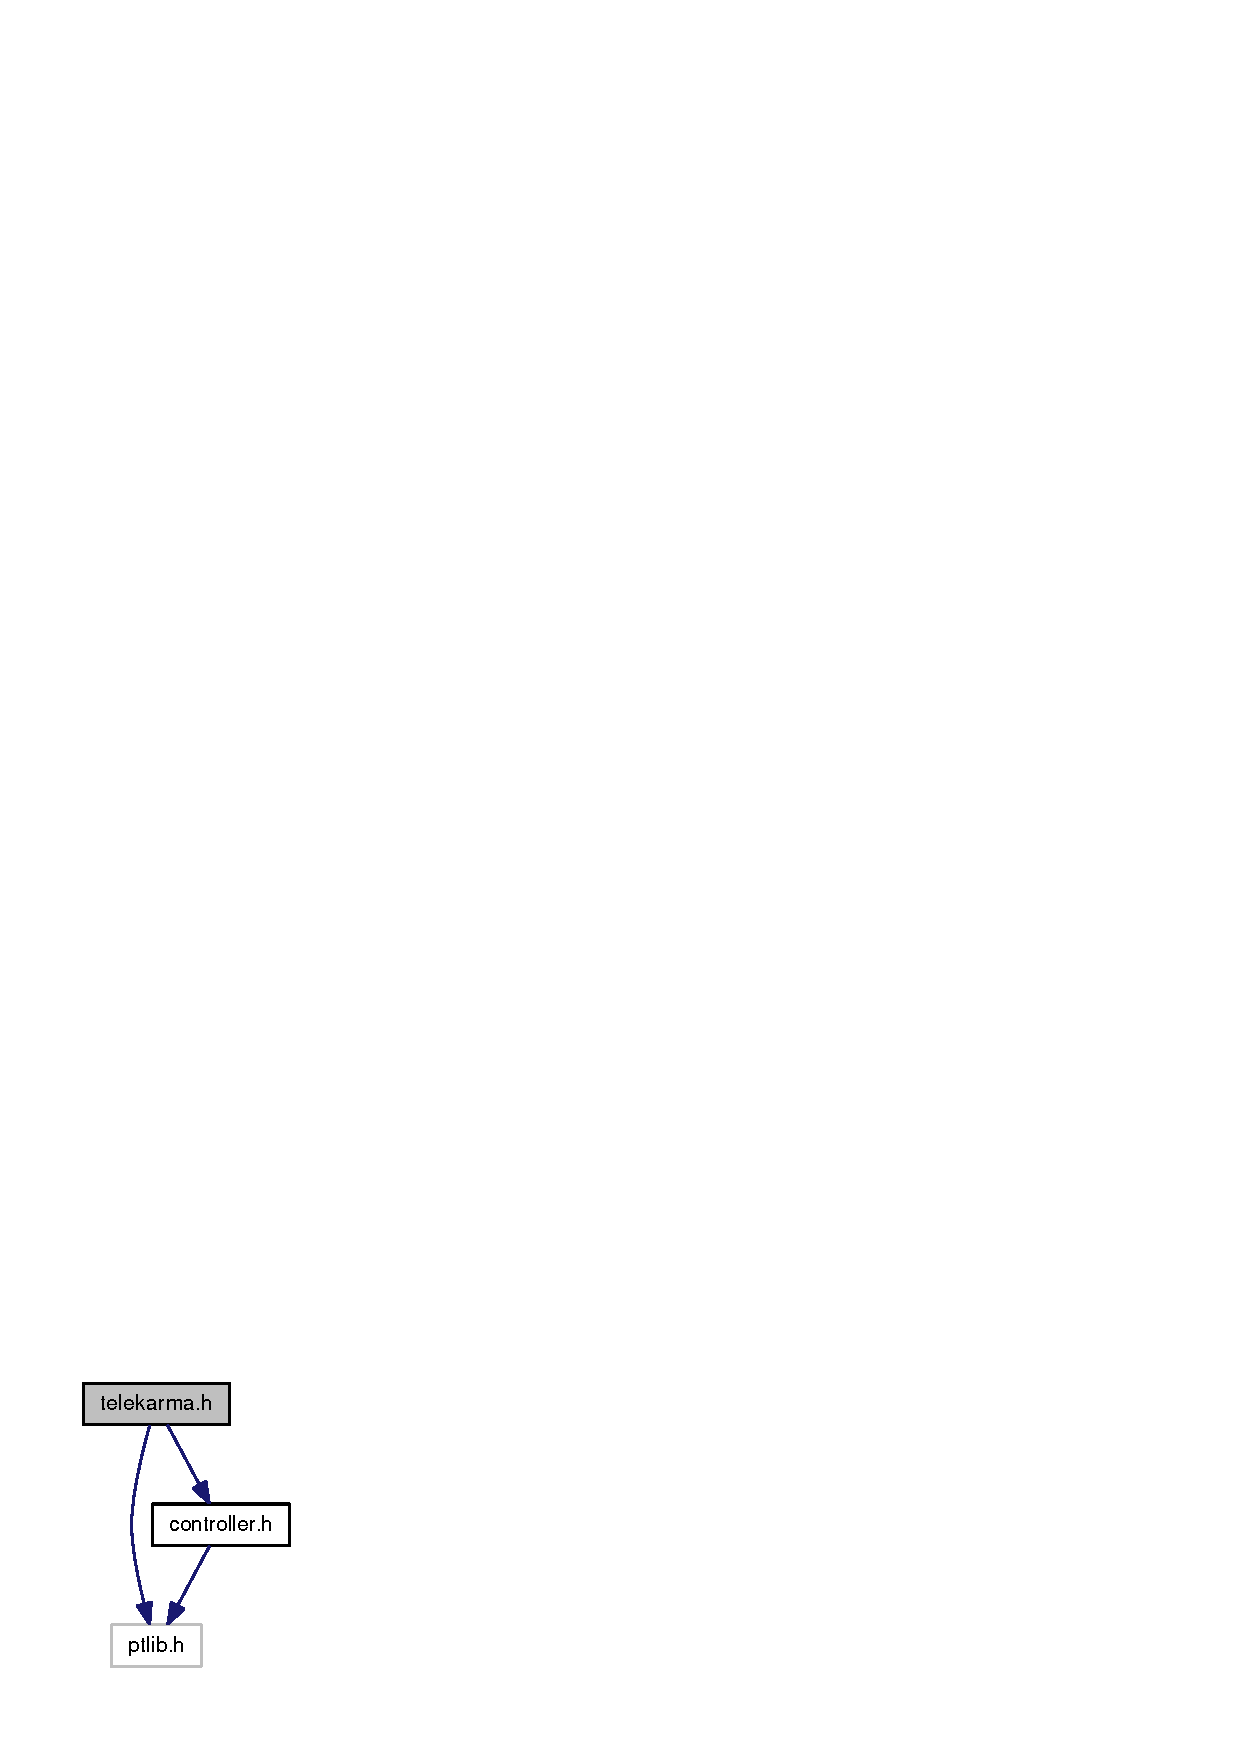
\includegraphics[width=71pt]{telekarma_8h__incl}
\end{center}
\end{figure}


This graph shows which files directly or indirectly include this file:\nopagebreak
\begin{figure}[H]
\begin{center}
\leavevmode
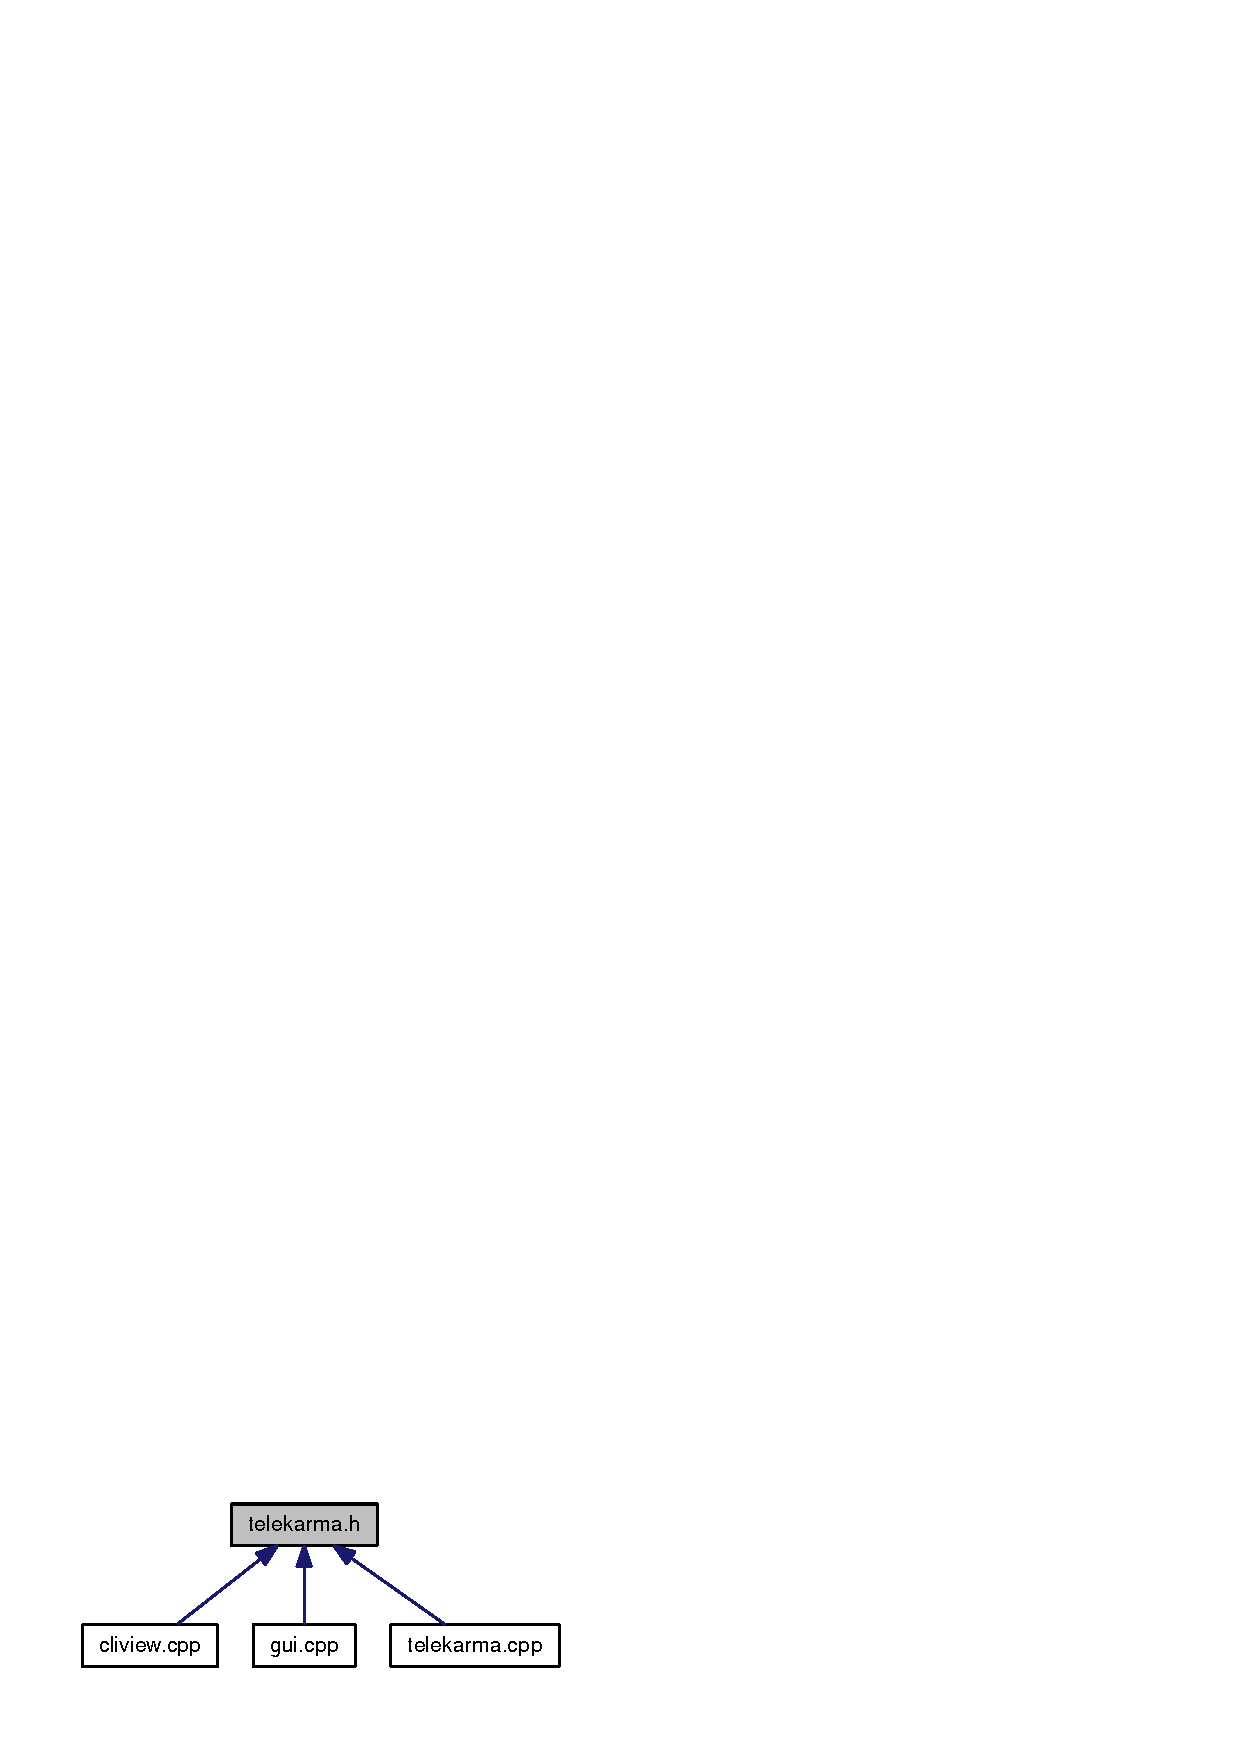
\includegraphics[width=136pt]{telekarma_8h__dep__incl}
\end{center}
\end{figure}
\subsection*{Classes}
\begin{CompactItemize}
\item 
class \hyperlink{classTeleKarma}{TeleKarma}
\end{CompactItemize}
\subsection*{Defines}
\begin{CompactItemize}
\item 
\#define \hyperlink{telekarma_8h_4af2a8a383f07fec0d9f78f2db1c987a}{SLEEP\_\-DURATION}~50
\begin{CompactList}\small\item\em Defines the minimum amount of time, in milliseconds, for the \hyperlink{classTeleKarma}{TeleKarma} main application thread to sleep between control loop iterations. \item\end{CompactList}\item 
\#define \hyperlink{telekarma_8h_e0edb34f25808edbd9c240ce645d36db}{PAUSE\_\-TIME}~0
\begin{CompactList}\small\item\em Defines the amount of dead time between iterations of audio file playback when in hold and human detection hold modes. \item\end{CompactList}\item 
\#define \hyperlink{telekarma_8h_6d87d074354c891b4bf9847003bc6be7}{IVR\_\-REPEATS}~10000
\begin{CompactList}\small\item\em Defines the number of times an audio file should be played, at most, while in hold and human detection hold modes. \item\end{CompactList}\item 
\#define \hyperlink{telekarma_8h_36554d6c57b18df85466ed9424676b16}{EXIT\_\-DELAY}~1000
\begin{CompactList}\small\item\em Defines how long to wait to close the program after initiating termination. \item\end{CompactList}\item 
\#define \hyperlink{telekarma_8h_a2c5891331d3c285a8705be0397c92af}{IS\_\-HUMAN\_\-TONE}~'1'
\begin{CompactList}\small\item\em Defines which DTMF tone (using the associated key label) that is interpreted to mean that the remote party is a human while in human detection hold mode. \item\end{CompactList}\item 
\#define \hyperlink{telekarma_8h_5958fe3d2eaf64cc44c7f0ecdcde5a3c}{AUTO\_\-HOLD\_\-WAV}~\char`\"{}press1.wav\char`\"{}
\begin{CompactList}\small\item\em Defines the filename and path (relative to the telekarma executable file's location) of the audio file played to the remote party while in human detection hold mode. \item\end{CompactList}\item 
\#define \hyperlink{telekarma_8h_491b1ae757a7494b35cdd4e58aa3fe0a}{HOLD\_\-WAV}~\char`\"{}pleasehold.wav\char`\"{}
\begin{CompactList}\small\item\em Defines the filename and path (relative to the telekarma executable file's location) of the audio file played to the remote party while in standard hold mode. \item\end{CompactList}\item 
\#define \hyperlink{telekarma_8h_79b9c64188ba6b1ebd310a44ad46ddb8}{REGISTRATION\_\-TIMEOUT}~(10$\ast$1000)
\begin{CompactList}\small\item\em Defines the minimum timeout duration in milliseconds for registration. \item\end{CompactList}\end{CompactItemize}


\subsection{Define Documentation}
\hypertarget{telekarma_8h_5958fe3d2eaf64cc44c7f0ecdcde5a3c}{
\index{telekarma.h@{telekarma.h}!AUTO\_\-HOLD\_\-WAV@{AUTO\_\-HOLD\_\-WAV}}
\index{AUTO\_\-HOLD\_\-WAV@{AUTO\_\-HOLD\_\-WAV}!telekarma.h@{telekarma.h}}
\subsubsection[{AUTO\_\-HOLD\_\-WAV}]{\setlength{\rightskip}{0pt plus 5cm}\#define AUTO\_\-HOLD\_\-WAV~\char`\"{}press1.wav\char`\"{}}}
\label{telekarma_8h_5958fe3d2eaf64cc44c7f0ecdcde5a3c}


Defines the filename and path (relative to the telekarma executable file's location) of the audio file played to the remote party while in human detection hold mode. 

The audio contained in this file should ask the remote party to press the key defined by IS\_\-HUMAN\_\-TONE. Brevity is desireable in the audio clip. Format: PCM-16 8Khz Mono WAV. \hypertarget{telekarma_8h_36554d6c57b18df85466ed9424676b16}{
\index{telekarma.h@{telekarma.h}!EXIT\_\-DELAY@{EXIT\_\-DELAY}}
\index{EXIT\_\-DELAY@{EXIT\_\-DELAY}!telekarma.h@{telekarma.h}}
\subsubsection[{EXIT\_\-DELAY}]{\setlength{\rightskip}{0pt plus 5cm}\#define EXIT\_\-DELAY~1000}}
\label{telekarma_8h_36554d6c57b18df85466ed9424676b16}


Defines how long to wait to close the program after initiating termination. 

Longer values give users more time to read the console and thus understand why the program is exiting. \hypertarget{telekarma_8h_491b1ae757a7494b35cdd4e58aa3fe0a}{
\index{telekarma.h@{telekarma.h}!HOLD\_\-WAV@{HOLD\_\-WAV}}
\index{HOLD\_\-WAV@{HOLD\_\-WAV}!telekarma.h@{telekarma.h}}
\subsubsection[{HOLD\_\-WAV}]{\setlength{\rightskip}{0pt plus 5cm}\#define HOLD\_\-WAV~\char`\"{}pleasehold.wav\char`\"{}}}
\label{telekarma_8h_491b1ae757a7494b35cdd4e58aa3fe0a}


Defines the filename and path (relative to the telekarma executable file's location) of the audio file played to the remote party while in standard hold mode. 

Brevity is desireable in the audio clip. Format: PCM-16 8Khz Mono WAV. \hypertarget{telekarma_8h_a2c5891331d3c285a8705be0397c92af}{
\index{telekarma.h@{telekarma.h}!IS\_\-HUMAN\_\-TONE@{IS\_\-HUMAN\_\-TONE}}
\index{IS\_\-HUMAN\_\-TONE@{IS\_\-HUMAN\_\-TONE}!telekarma.h@{telekarma.h}}
\subsubsection[{IS\_\-HUMAN\_\-TONE}]{\setlength{\rightskip}{0pt plus 5cm}\#define IS\_\-HUMAN\_\-TONE~'1'}}
\label{telekarma_8h_a2c5891331d3c285a8705be0397c92af}


Defines which DTMF tone (using the associated key label) that is interpreted to mean that the remote party is a human while in human detection hold mode. 

The audio file played while in human detection hold mode should ask the remote party to press this key. \hypertarget{telekarma_8h_6d87d074354c891b4bf9847003bc6be7}{
\index{telekarma.h@{telekarma.h}!IVR\_\-REPEATS@{IVR\_\-REPEATS}}
\index{IVR\_\-REPEATS@{IVR\_\-REPEATS}!telekarma.h@{telekarma.h}}
\subsubsection[{IVR\_\-REPEATS}]{\setlength{\rightskip}{0pt plus 5cm}\#define IVR\_\-REPEATS~10000}}
\label{telekarma_8h_6d87d074354c891b4bf9847003bc6be7}


Defines the number of times an audio file should be played, at most, while in hold and human detection hold modes. 

The aim here is for essentially endless playback looping, so this number should be large. \hypertarget{telekarma_8h_e0edb34f25808edbd9c240ce645d36db}{
\index{telekarma.h@{telekarma.h}!PAUSE\_\-TIME@{PAUSE\_\-TIME}}
\index{PAUSE\_\-TIME@{PAUSE\_\-TIME}!telekarma.h@{telekarma.h}}
\subsubsection[{PAUSE\_\-TIME}]{\setlength{\rightskip}{0pt plus 5cm}\#define PAUSE\_\-TIME~0}}
\label{telekarma_8h_e0edb34f25808edbd9c240ce645d36db}


Defines the amount of dead time between iterations of audio file playback when in hold and human detection hold modes. 

In these modes, audio files are played in a repeating loop. \hypertarget{telekarma_8h_79b9c64188ba6b1ebd310a44ad46ddb8}{
\index{telekarma.h@{telekarma.h}!REGISTRATION\_\-TIMEOUT@{REGISTRATION\_\-TIMEOUT}}
\index{REGISTRATION\_\-TIMEOUT@{REGISTRATION\_\-TIMEOUT}!telekarma.h@{telekarma.h}}
\subsubsection[{REGISTRATION\_\-TIMEOUT}]{\setlength{\rightskip}{0pt plus 5cm}\#define REGISTRATION\_\-TIMEOUT~(10$\ast$1000)}}
\label{telekarma_8h_79b9c64188ba6b1ebd310a44ad46ddb8}


Defines the minimum timeout duration in milliseconds for registration. 

\hypertarget{telekarma_8h_4af2a8a383f07fec0d9f78f2db1c987a}{
\index{telekarma.h@{telekarma.h}!SLEEP\_\-DURATION@{SLEEP\_\-DURATION}}
\index{SLEEP\_\-DURATION@{SLEEP\_\-DURATION}!telekarma.h@{telekarma.h}}
\subsubsection[{SLEEP\_\-DURATION}]{\setlength{\rightskip}{0pt plus 5cm}\#define SLEEP\_\-DURATION~50}}
\label{telekarma_8h_4af2a8a383f07fec0d9f78f2db1c987a}


Defines the minimum amount of time, in milliseconds, for the \hyperlink{classTeleKarma}{TeleKarma} main application thread to sleep between control loop iterations. 

